%{{{-----------------------------------Basics----------------------------------%

%document class definition
\documentclass[
    11pt,
    a4paper,
    oneside,
    headinlcude, footinclude,
    twoside,
]{report}


%essential packages
\renewcommand*\rmdefault{ppl}
\usepackage[top=2.5cm,bottom=2cm,left=3cm,right=3cm]{geometry}
\usepackage[english]{babel}
\usepackage[T1]{fontenc}
\usepackage[utf8]{inputenc}
\usepackage{xcolor}
\usepackage{amssymb}


%additional packages
\usepackage{amsmath}
\usepackage[framemethod=Tikz]{mdframed}
\usepackage{tikz}
\usepackage{enumerate}
\usepackage{graphicx}
\usepackage{pgf,tikz,pgfplots} % for the transfer from geogebra to tikz
\usepackage{mathrsfs}% for the transfer from geogebra to tikz
\usepackage{wrapfig}
\usepackage{fancyhdr}
\usepackage{tabularx}
\usepackage{makecell} % to make thick hlines in the front page

%}}}

%{{{-----------------------------------Macros----------------------------------%

\newcommand{\myImplies}[0]{\rightarrow}

\newcommand{\powerset}[1]{\mathcal{P}(#1)}

\newcommand{\tvect}[3]{%
   \ensuremath{\Bigl(\begin{smallmatrix}#1\\#2\\#3\end{smallmatrix}\Bigr)}}

\newcommand{\myVector}[3]{\begin{pmatrix}#1\\#2\\#3\end{pmatrix}}

\newcommand{\myVectorII}[2]{\begin{pmatrix}#1\\#2\end{pmatrix}}

\newcommand{\ssi}[0]{\Longleftrightarrow}

\newcommand{\markDate}[1]{\begin{flushright}#1\end{flushright}}

\renewcommand{\vec}[1]{\overrightarrow{#1}}

\def\getangle(#1)(#2)#3{
    \begingroup
        \pgftransformreset
        \pgfmathanglebetweenpoints{\pgfpointanchor{#1}{center}}{\pgfpointanchor{#2}{center}}
        \expandafter\xdef\csname angle#3\endcsname{\pgfmathresult}
    \endgroup
}

\newcommand{\tq}[0]{ \ \textrm{t.q.}\ }

\newcommand\Warning{
    \makebox[1.4em][c]{
    \makebox[-5.5pt][c]{\raisebox{.2em}{!}}
    \makebox[0pt][c]{\color{red}\huge$\bigtriangleup$}}
}

%colored frame box
\newcommand{\cfbox}[2]{
    \colorlet{currentcolor}{.}
    {\color{#1}
    \fbox{\color{currentcolor}#2}}
}


%}}}

%{{{----------------------------------Settings---------------------------------%

\title{Maths 2A - Géometrie vectorielle}

\author{Arno Fauconnet}

\setlength{\parindent}{0pt} %disable initial indent on first paragraph of sections in the whole doc

% the style of the boxes
\newmdenv[
        roundcorner=10pt,
        middlelinecolor=red,
        backgroundcolor=gray!15,
        linewidth=2pt,
        frametitlerule=true]{highlightBox}

% increases the space between paragraphs
\setlength{\parskip}{.3em}

\usetikzlibrary{calc}
\usetikzlibrary{arrows}%for the transfer from geogebra to tikz


% Geogebras wierd colors xD
\definecolor{qqqqff}{rgb}{0.,0.,1.}
\definecolor{ffqqtt}{rgb}{1.,0.,0.2}
\definecolor{ududff}{rgb}{0.30196078431372547,0.30196078431372547,1.} 
\definecolor{ffqqqq}{rgb}{1.,0.,0.} 
\definecolor{xdxdff}{rgb}{0.49019607843137253,0.49019607843137253,1.}
\definecolor{zzttqq}{rgb}{0.6,0.2,0.}
\definecolor{uuuuuu}{rgb}{0.26666666666666666,0.26666666666666666,0.26666666666666666}
\definecolor{wwccff}{rgb}{0.4,0.8,1.}
\definecolor{qqzzff}{rgb}{0.,0.6,1.}
\definecolor{qqzzqq}{rgb}{0.,0.6,0.}

\tikzstyle{every node}=[font=\large]


\graphicspath{ {Maths_2A/figures/} }


% header and footer settings
\pagestyle{fancy}
\fancyhf{}
\fancyhead[LE,LO]{Arnaud Fauconnet}
\fancyhead[CE,CO]{\textsc{Maths 2A}}
\fancyhead[RE,RO]{MAN - Printemps 2019}
\fancyfoot[CE,CO]{\leftmark}
\fancyfoot[LE,RO]{\thepage}

\renewcommand{\headrulewidth}{2pt}
\renewcommand{\footrulewidth}{1pt}
%}}}

%%%%%%%%%%%%%%%%%%%%%%%%%%%%%%%%%%%%%%%%%%%%%%%%%%%%%%%%%%%%%%%%%%%%%%%%%%%%%%
%----------------------------------------------------------------------------%
%-------------------------------Text starts here-----------------------------%
%----------------------------------------------------------------------------%
%%%%%%%%%%%%%%%%%%%%%%%%%%%%%%%%%%%%%%%%%%%%%%%%%%%%%%%%%%%%%%%%%%%%%%%%%%%%%%


\begin{document}

\begin{titlepage}
   \begin{center}
       \vspace*{\fill}

       {\Huge EPFL}\\ 
%----------------------------------------------------------------------------%
       \vfill
       {\huge MAN}\\ [1em]
       {\Large Mise à niveau}\\
%----------------------------------------------------------------------------%
        \vfill
        \begin{tabularx}{\textwidth}{X}
            \Xhline{3\arrayrulewidth}\\
        \end{tabularx}\\ [2em]
        {\Huge Maths 2A} \\ [1em]
        \textsc{\huge Prepa-032(a)} \\ [2em]
        \begin{tabularx}{\textwidth}{X}
            \Xhline{3\arrayrulewidth}\\
        \end{tabularx}\\ [2em]
%----------------------------------------------------------------------------%
        \vspace{.7cm}
        {\large
        \begin{tabularx}{.9\textwidth}{Xr}
            \textit{Student:} & \textit{Professor:}\\
            Arnaud \textsc{Fauconnet} & Sacha \textsc{Friedly}
        \end{tabularx}}
%----------------------------------------------------------------------------%
        \vfill
        {\Large Printemps - 2019}

%----------------------------------------------------------------------------%
        \vfill
        \includegraphics[width=7cm]{epfl-logo}

       \vfill
   \end{center} 
\end{titlepage} 
\setcounter{chapter}{0}
\chapter{Vecteurs \& opération}
\markDate{25/02/2019}

Motivations:

\begin{enumerate}
    \item Forces:

        \hspace*{4cm}
        \begin{tikzpicture}[scale=1.4]
            \draw (0,0) -- (2, 0);
            \draw (0.5, 0) -- (.5, .75) -- (1.5, .75) -- (1.5, 0);
            \draw [->] (1, .35) -- (1, 1.25) node[anchor=west] {$\vec N$};
            \draw [->] (1, .25) -- (1, -.75) node[anchor=west] {$\vec P$};
            \draw [->] (1, .3) -- (2, .3) node[anchor=west] {$\vec V$};
        \end{tikzpicture}

    \item Déplacements:

        \hspace*{4cm}
        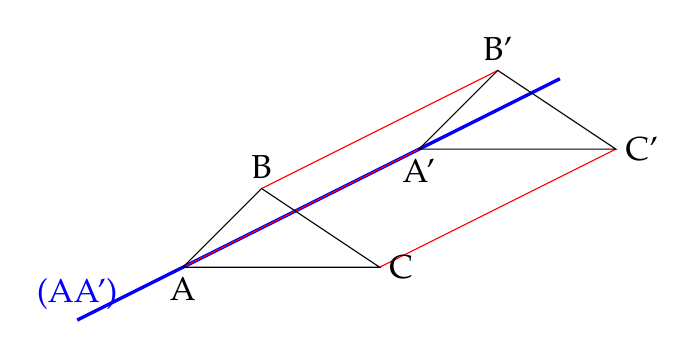
\begin{tikzpicture}
            \def\deplx{3}
            \def\deply{1.5}

            \coordinate (A) at (0, 0) {};
            \coordinate (B) at (1, 1) {};
            \coordinate (C) at (2.5, 0) {};

            \coordinate (A1) at (0+\deplx, 0+\deply) {};
            \coordinate (B1) at (1+\deplx, 1+\deply) {};
            \coordinate (C1) at (2.5+\deplx, 0+\deply) {};

            \draw [very thick, blue] ($(A)!-1.5cm!(A1)$) node[anchor=south] {(AA')}-- ($(A1)!-2cm!(A)$);

            \draw [red] (A) -- (A1);
            \draw [red] (B) -- (B1);
            \draw [red] (C) -- (C1);

            \draw (A) node [anchor=north] {A} -- (B) node [anchor=south] {B} -- (C) node [anchor=west] {C} -- cycle;
            \draw (A1) node [anchor=north] {A'} -- (B1) node [anchor=south] {B'} -- (C1) node [anchor=west] {C'} -- cycle;
        \end{tikzpicture}

        Segements: $AA' \neq BB' \neq CC'$ \\
        Droites: $(AA') \parallel (BB') \parallel (CC')$ \\
        Vecteurs: $\overrightarrow{AA'} = \overrightarrow{BB'} = \overrightarrow{CC'}$ 
\end{enumerate}

Dans le plan ou l'espace, un vecteur est définie par:
\begin{enumerate}
    \item une \textbf{direction}: "une" droite qui porte le vecteur
    \item une \textbf{longueur}/\textbf{norme} 
    \item un \textbf{sens} 
\end{enumerate}

Bonne façon de penser: des flèches.

(Si on se fixe une origine: Ensemble des vecteurs $\implies$ Espace vectoriels)

\vspace{.5cm}

\textbf{Conventions:}

On notera les vecteurs : $\vec a, \vec b, \vec c, ..., \vec u, \vec v, \vec w$\\
La \underline{norme} de $\vec a$: $\| \vec a \| \geq 0$ (avec choix d'\textbf{unité}!)\\
Le vecteur nul: $\vec 0 \quad \| \vec 0 \| = 0$


\section{Addition vectorielle}
\label{sec:addition_vectorielle}

Motivation:

\begin{enumerate}
    \item En physique:
       
        \hspace*{4cm}
        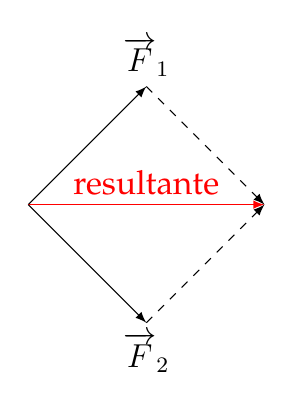
\begin{tikzpicture}[>=latex, scale=.75]
            \draw [->] (0, 0) -- (2, 2) node[anchor=south] {$\vec F_{1}$};
            \draw [->, red] (0, 0) -- (4, 0);
            \draw [->] (0, 0) -- (2, -2) node[anchor=north] {$\vec F_{2}$};

            \node [anchor=south, red] at (2, 0) {resultante};

            \draw [dashed, ->] (2, 2) -- (4, 0);
            \draw [dashed, ->] (2, -2) -- (4, 0);
        \end{tikzpicture}

    \item Déplacements:

        \hspace*{4cm}
        \begin{tikzpicture}[>=latex]
            \def\deplx{3}
            \def\deply{1.5}
            \def\deplxi{5}
            \def\deplyi{-1}

            \coordinate (A) at (0, 0) {};
            \coordinate (B) at (1, 1) {};
            \coordinate (C) at (2.5, 0) {};
            \coordinate (center) at (1.166, .33) {};

            \coordinate (A1) at (0+\deplx, 0+\deply) {};
            \coordinate (B1) at (1+\deplx, 1+\deply) {};
            \coordinate (C1) at (2.5+\deplx, 0+\deply) {};
            \coordinate (center1) at (1.166+\deplx, .33+\deply) {};

            \coordinate (A2) at (0+\deplxi, 0+\deplyi) {};
            \coordinate (B2) at (1+\deplxi, 1+\deplyi) {};
            \coordinate (C2) at (2.5+\deplxi, 0+\deplyi) {};
            \coordinate (center2) at (1.166+\deplxi, .33+\deplyi) {};

            \getangle(center)(center2)a;

            \draw (A) -- (B) -- (C) -- cycle;
            \draw (A) -- (B) -- (C) -- cycle;
            \draw (A) -- (B) -- (C) -- cycle;

            \draw (A1) -- (B1) -- (C1) -- cycle;
            \draw (A1) -- (B1) -- (C1) -- cycle;
            \draw (A1) -- (B1) -- (C1) -- cycle;

            \draw (A2) -- (B2) -- (C2) -- cycle;
            \draw (A2) -- (B2) -- (C2) -- cycle;
            \draw (A2) -- (B2) -- (C2) -- cycle;

            \draw [red, ->] (center) -- (center1) node [midway, red, anchor=south] {$\vec v$};
            \draw [blue, ->] (center1) -- (center2) node [midway, blue, anchor=south] {$\vec w$};
            \draw [green, ->] (center) -- (center2) node [midway, green, above, rotate=\anglea] {resultante};
        \end{tikzpicture}
\end{enumerate}

L'\textbf{addition} de deux vecteurs $\vec a , \vec b$ est définie par
\underline{la règle du parallelogramme}.

\begin{center}
    \begin{tikzpicture}[scale=1, transform shape]
        \coordinate (A) at (0, 0);
        \coordinate (B) at (5, 2);

        \getangle(A)(B)a;

        \draw [->] (0, 0) -- (4, 0) node [midway, anchor=north] {$\vec a$};
        \draw [->] (0, 0) -- (1, 2) node [midway, anchor=east] {$\vec b$};

        \draw [->, dashed] (1, 2) -- (5, 2);
        \draw [->, dashed] (4, 0) -- (5, 2);

        \draw [->, red] (0, 0) -- (5, 2) node [midway, above, rotate=\anglea] {$\vec a + \vec b$};
    \end{tikzpicture}
\end{center}

\paragraph{Propriétés} 
\begin{itemize}
    \item $\vec a + \vec b = \vec b + \vec a$
    \item $(\vec a + \vec b) + \vec c = \vec a + (\vec b + \vec c)$
    \item $\vec a + \vec 0 = \vec a$
    \item $\forall \vec a, \exists! \vec a'\tq\vec a + \vec a' = \vec 0$

        On notera $\vec a' = - \vec a$ (appelé \textbf{opposé} de $\vec a$)
\end{itemize}

\pagebreak

On peut définir une \textbf{soustraction}:

$$ \vec a - \vec b := \vec a + (- \vec b) $$

\begin{center}
\begin{tikzpicture}[transform shape]
    \coordinate (A) at (0, 0);
    \coordinate (B) at (5, 2);
    \coordinate (C) at (3, -2);

    \getangle(A)(B)a;
    \getangle(A)(C)b;

    \draw [->] (0, 0) -- (4, 0) node [midway, anchor=north] {$\vec a$};
    \draw [->] (0, 0) -- (1, 2) node [midway, anchor=east] {$\vec b$};

    \draw [->, dashed] (1, 2) -- (5, 2);
    \draw [->, dashed] (4, 0) -- (5, 2);

    \draw [->] (0, 0) -- (5, 2) node [midway, above, rotate=\anglea] {$\vec a + \vec b$};

    \draw [->, red] (0, 0) -- (-1, -2) node [midway, anchor=east, red] {$\vec b$};
    \draw [->, dashed, red] (-1, -2) -- (3, -2);
    \draw [->, dashed, red] (4, 0) -- (3, -2);

    \draw [->, red] (0, 0) -- (3, -2) node [midway, below, rotate=\angleb] {$\vec a + \vec b$};
\end{tikzpicture}
\end{center}

\paragraph{Une formulation de la règle du parallelogramme}
\begin{center}
    \begin{tikzpicture}
        \coordinate (A) at (0, 0);
        \coordinate (B) at (3, 3);
        \coordinate (C) at (6, 0);

        \getangle(A)(B)a;
        \getangle(B)(C)b;

        \node [anchor=east] at (A) {A};
        \node [anchor=south] at (B) {B};
        \node [anchor=west] at (C) {C};

        \draw [->] (A) -- node [midway,above,rotate=\anglea] {$\vec{AB}$} (B);
        \draw [->] (B) -- node [midway,above,rotate=\angleb] {$\vec{BC}$} (C);
        \draw [->] (A) -- node [midway,below] {$\vec{AC}$} (C);
    \end{tikzpicture}
\end{center}

\begin{highlightBox}[frametitle={Règle de Chasles}]
    \begin{equation}
        \label{eq:1}
        \vec{AB} + \vec{BC} = \vec{AC}
    \end{equation}
\end{highlightBox}

\textbf{Remarque:} 

\begin{enumerate}
    \item On peut l'iterer:
        \begin{center}
            \begin{tikzpicture}[>=latex]
                \draw [red, ->] (0, 0) node [anchor=east] {$A_{1}$} -- (8, -1) node [anchor=west] {$A_{n}$};
                \draw [->] (0, 0) -- (3, 2) node [anchor=south] {$A _{2}$};
                \draw [->] (3, 2) -- (4, -3) node [anchor=north] {$A _{3}$};
                \draw [->] (4, -3) -- (6, 2) node [anchor=south] {$A _{4}$};
                \draw [->] (6, 2) -- (8, -1);
            \end{tikzpicture}
        \end{center}

        Pour les points $A_{1}, ..., A_{n}$

        $$\vec{A_{1} A_{n}} = \vec{A_{1} A_{2}} + \vec{A_{2} A_{3}} + ... + \vec{A_{n-1} A_{n}}$$

    \item Si $A = C$ dans (\ref{eq:1}):

        \begin{equation}
            \begin{split}
                \vec{AB} + \vec{BA} = \vec{AA} = \vec 0 
                \\ 
                \implies \vec{BA} = -\vec{AB} 
            \end{split}
        \end{equation}

    \item $\vec{AB} + \vec{BC} = \vec{AC}$ n'implique pas (en général) $\|\vec{AB}\| + \|\vec{BC}\| = \|\vec{AC}\|$

        En fait a l'\textbf{inegalité triangle}:
        \begin{highlightBox}[frametitle={Inegalité triangle}]
            \center
                $\|\vec{AC}\| \leq \|\vec{AB}\| + \|\vec{BC}\|$
        \end{highlightBox}
\end{enumerate}

\section{Multiplication par un scalaire}
\label{sec:multiplication_par_un_scalaire}

Si $\vec a$ est un vecteur et $\lambda \in \mathbb{R}$ (un scalaire), on
définit $\lambda \vec a$ comme suit:

\begin{itemize}
    \item Si $\lambda = 0$, alors $\lambda \vec a := \vec 0$
    \item Si $\lambda \neq 0$, alors $\lambda \vec a$ a même direction

       $\hookrightarrow$  Si $\lambda > 0, \lambda \vec a$ le même sens que $\vec a$\\
       $\hookrightarrow$  Si $\lambda < 0, \lambda \vec a$ est de sens opposée à $\vec a$

       $\implies \lambda \vec a$ a longueur $\| \lambda \vec a \| = | \lambda
       | \| \vec a \|$
\end{itemize}

\paragraph{Exemple} 
$\lambda = \frac{3}{2}$

\begin{center}
    \begin{tikzpicture}[>=latex]
        \coordinate (A) at (0, 0);
        \coordinate (B) at (2, 2);
        \getangle(A)(B)a
        \draw [->] (A) -- (B) node [midway, below, rotate=\anglea] {$\vec
        a$};
        \draw [->, red] (0, 0.1) -- (3, 3.1) node [midway, above, rotate=\anglea] {$\lambda \vec a$};
;
    \end{tikzpicture}
\end{center}

\begin{highlightBox}[frametitle={Propriétés}]
    \begin{enumerate}
        \item $\lambda \vec a = \vec 0 \iff \vec a = \vec 0 \ \textrm{ou}\ \lambda = 0$
        \item $1 \vec a = \vec a,  (-1) \vec a = - \vec a$
        \item $\lambda (\mu \vec a) = \mu (\lambda \vec a) = (\mu\lambda)\vec a$
        \item $\lambda (\vec a + \vec b) = \lambda \vec a + \lambda \vec b$
        \item $(\lambda + \mu) \vec a = \lambda \vec a + \mu \vec a$
    \end{enumerate}
\end{highlightBox}

(Muni de "+" et de la multiplicatoin par des scalaires, les vecteurs forment
un espace vectoriel)

On peut maintenant résoudre des equations:

$$ 2 \vec x + \vec b = \vec c - \vec x$$

\pagebreak 

\section{"Vectorisation" de la géométrie}

\begin{enumerate}
    \item $A, B, C$ sont alignés $\iff \exists \lambda \in \mathbb{R} \tq\vec{AB}
        = \lambda \vec{AC}$

        \begin{center}
            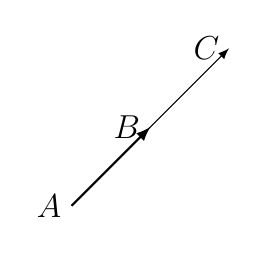
\begin{tikzpicture}[>=latex]
                \draw [->, thick] (0, 0) node[anchor=east] {$A$} -- (1, 1) node [anchor=east] {$B$};
                \draw [->] (0, 0) -- (2, 2) node [anchor=east] {$C$};
            \end{tikzpicture}
        \end{center}

        \textbf{Remarque:} 

        \begin{center}
            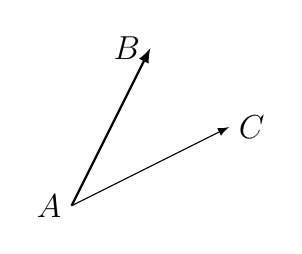
\begin{tikzpicture}[>=latex, scale=2]
                \draw [->, thick] (0, 0) node[anchor=east] {$A$} -- (.5, 1) node [anchor=east] {$B$};
                \draw [->] (0, 0) -- (1, .5) node [anchor=west] {$C$};
            \end{tikzpicture}
        \end{center}

        Les points si-dessus ne sont pas alignés: 
        $\nexists \lambda \in \mathbb{R} \tq\vec{AB} = \lambda \vec{AC}$

    \item 4 poitns = $A, B, C, D$ froment un parallelogramme $\iff \vec{AB} =
        \pm \vec{DC}$, ou $\vec{AD} \pm \vec{BC}$, ou $\vec{AC} = \pm \vec{BD}$
\end{enumerate}

\textbf{Theoremes} 

\begin{enumerate}
    \item \textbf{Theorème (Vargninon)}: Les milieux des côtés d'un
        quadrilatère quelconque forment un parallelogramme.

        \begin{center}
            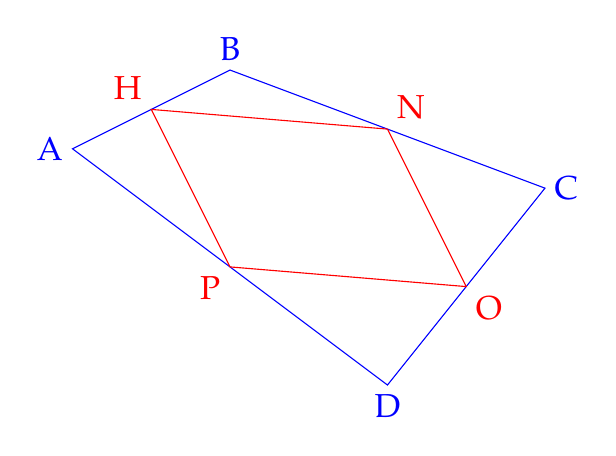
\begin{tikzpicture}
                \coordinate (A) at (0, 0);
                \coordinate (B) at (2, 1);
                \coordinate (C) at (6, -.5);
                \coordinate (D) at (4, -3);

                \draw [blue] (A) node[anchor=east] {A} -- coordinate[midway](c1) (B) node[anchor=south] {B} -- coordinate[midway](c2) (C) node[anchor=west] {C} -- coordinate[midway](c3) (D) node[anchor=north] {D} -- coordinate[midway](c4) cycle;

                \draw [red] (c1) node[anchor=south east] {H} -- (c2) node[anchor=south west] {N} -- (c3) node[anchor=north west] {O} -- (c4) node[anchor=north east] {P} -- cycle;
            \end{tikzpicture}
        \end{center}

        \underline{Preuve:} À voir $\vec{MC} = \vec{PO}$


        \[
            \begin{split}
                \vec{MN} = \vec{MB} + \vec{BN} \\ 
                =  \frac{1}{2}\vec{AB} + \frac{1}{2}\vec{BC} \\
                =  \frac{1}{2}(\vec{AB} + \vec{BC}) = \frac{1}{2}\vec{AC}
            \end{split}
        \]

        \pagebreak 

        De même:

        $$ \vec{PO} = ... = \frac{1}{2} \vec{AC} $$

        \[ 
            \begin{split}
                \implies \frac{1}{2} \vec{AC} = \frac{1}{2} \vec{AC}\\
                \implies \vec{MN} = \vec{PO}
            \end{split}
        \]

    \item \textbf{Theorème de Thalès} "version vectoriel"

        \begin{center}
            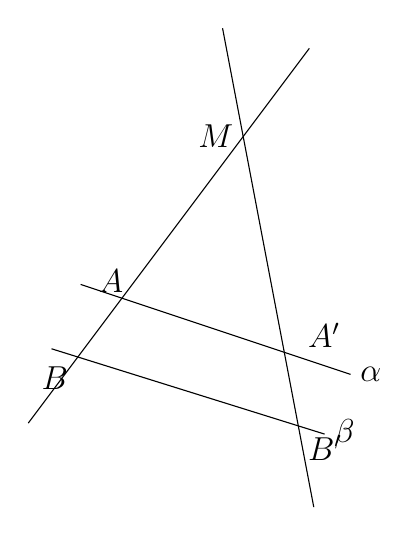
\begin{tikzpicture}[scale=.7]

                \coordinate (M) at (0, 0);
                \coordinate (A) at (-2, -3);
                \coordinate (A1) at (1, -4);

                \coordinate (B) at (-3, -4);
                \coordinate (B1) at (1, -5.25);

                \node [anchor=south east] at (A) {$A$};
                \node [anchor=south west] at (A1) {$A'$};
                \node [anchor=north east] at (B) {$B$};
                \node [anchor=north west] at (B1) {$B'$};
                \node [anchor=east] at (M) {$M$};

                \draw ($(B)!-1.5cm!(M)$) -- ($(M)!-2cm!(B)$);
                \draw ($(B1)!-1.5cm!(M)$) -- ($(M)!-2cm!(B1)$);

                \draw ($(A)!-1cm!(A1)$) -- ($(A1)!-1cm!(A)$) node [anchor=west] {$\alpha$};
                \draw ($(B)!-.5cm!(B1)$) -- ($(B1)!-.5cm!(B)$) node [anchor=west] {$\beta$};

            \end{tikzpicture}
        \end{center}

        \begin{equation}
            \label{eq:3}
            M, A, B \ \textrm{alignés}\ \implies \exists \lambda \tq \vec{MA} =
            \lambda \vec{MB} 
        \end{equation}

        \begin{equation}
            \label{eq:4}
            M, A', B' \ \textrm{alignés}\ \implies \exists \lambda' \tq \vec{MA'} =
            \lambda' \vec{MB'} 
        \end{equation}

        Thalès: $\lambda = \lambda'$

        \textbf{Remarque} 
        
        De (\ref{eq:3}): $\| \vec{MA} \| = |\lambda| \| \vec{MB} \|$\\
        De (\ref{eq:4}): $\| \vec{MA'} \| = |\lambda'| \| \vec{MB'} \|$
\end{enumerate}

\textbf{Preuve}  

\[
    \begin{split}
        \vec{MA} = \lambda \vec{MB} \\
        \vec{MA'} + \vec{A'A} = \lambda (\vec{MB'} + \vec{B'B})\\
        \underbrace{\vec{MA'}}_\text{$\lambda' \vec{MB'}$} - \lambda \vec{MB'}
        = \lambda \vec{B'B} - \underbrace{\vec{A'A}}_\text{comme $\vec{A'A} \parallel
        \vec{B'B}, \exists \mu \in \mathbb{R} \tq \vec{A'A} = \mu \vec{B'B}$}\\
        (\lambda - \lambda') \vec{MB} = (\lambda - \mu) \vec{B'B}
    \end{split}
\]

Si une de ces parenthèse est non-nulle, alors on pourrait écrire $\vec{MB}$,
come multiple de $\vec{B'B}$ (ou vice-versa), ce qui signifierait qu'ils sont
parallèles.

On a donc $\underbrace{\lambda - \lambda' = 0}_\text{$\lambda = \lambda'$}$ et 
$\underbrace{\lambda - \mu = 0}_\text{$\lambda = \mu$}$

\begin{flushright}
    $\Box$
\end{flushright}

\section{Repères}
\label{sub:reperes}

\paragraph{Définition}
\label{par:definition}

Un vecteur directeur d'une droite / d'un plan est n'importe quel vecteur
obtenu à partir de deux points $A, B$ sur cette droite / plan.

\begin{center}
    \begin{minipage}{.5\linewidth}
        \resizebox{\textwidth}{!}{
            \begin{tikzpicture}[line cap=round,line join=round,>=triangle 45,x=1.0cm,y=1.0cm]

            \clip(-10.459476902522171,-3.9007918650685593) rectangle (2.872371009111592,5.346317425448772);
            \draw [line width=2.pt,domain=-10.459476902522171:2.872371009111592] plot(\x,{(--14.033443409906939--2.771053838445815*\x)/3.0173697351965534});
            \draw [->,line width=2.pt,color=ffqqqq] (-6.775001613625693,-1.571054008301152) -- (-3.7576318784291396,1.1999998301446633);
            \draw [->,line width=2.pt,color=qqqqff] (-1.3388275809873473,3.4213507155503917) -- (-2.6469680298997558,2.219997242059404);
            \begin{scriptsize}
            \draw [fill=ududff] (-6.775001613625693,-1.571054008301152) circle (2.5pt);
            \draw[color=ududff] (-6.631317340521099,-1.350396017461948) node [anchor=south east] {$A $};
            \draw [fill=ududff] (-3.7576318784291396,1.1999998301446635) circle (2.5pt);
            \draw[color=ududff] (-3.7371055536999123,1.4719736328069377) node[anchor=south east] {$B$};
            \draw[color=black] (-9.084213145663876,-3.7622391731462685) node [anchor=south east]{$f$};
            \draw [fill=xdxdff] (-1.3388275809873473,3.4213507155503917) circle (2.5pt);
            \draw[color=xdxdff] (-1.3047360732863627,3.6682903788343615) node [anchor=south east]{$A'$};
            \draw [fill=xdxdff] (-2.6469680298997558,2.219997242059404) circle (2.5pt);
            \draw[color=xdxdff] (-2.618420855956972,2.4675003821745083) node [anchor=south east]{$B'$};
            \draw[color=ffqqqq] (-4.435000594493674,0.03513090176095963) node {$\vec{AB}$};
            \draw[color=qqqqff] (-0.8326306045141123,2.7856584154775463) node {$\vec{A'B'}$};
            \end{scriptsize}
            \end{tikzpicture}
        }
    \end{minipage}
    \begin{minipage}{.49\linewidth}
    L'ensemble des vecteurs d'une droite forment un espace vectoriel, de
    dimension $1$.
    \end{minipage}
\end{center}

\begin{minipage}{.5\linewidth}
    \resizebox{\textwidth}{!}{
        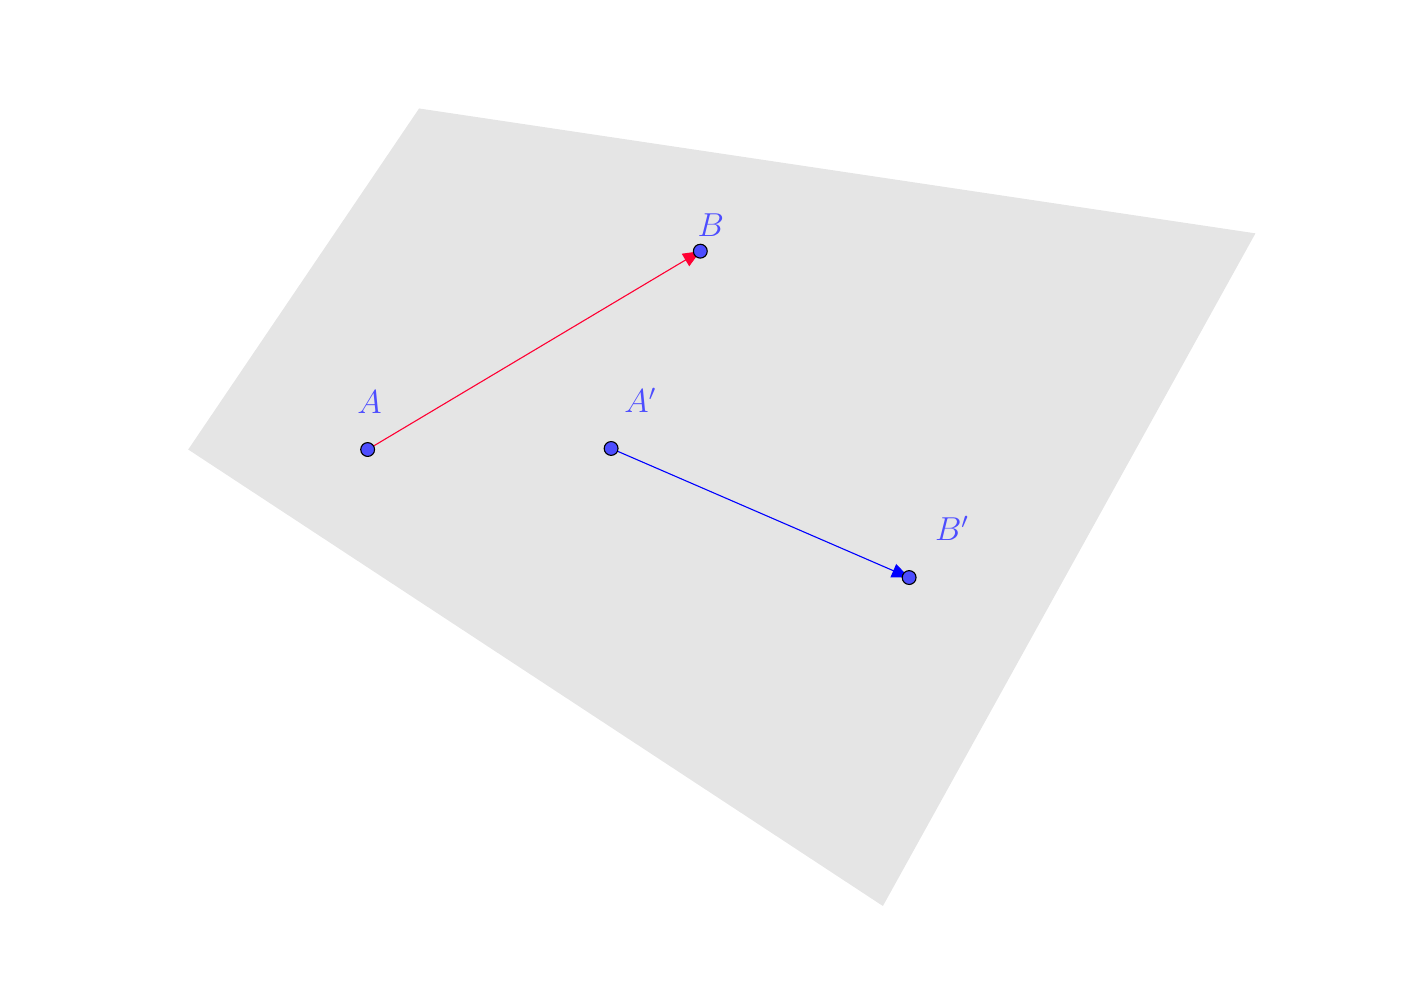
\begin{tikzpicture}[line cap=round,line join=round,>=triangle 45,x=1.0cm,y=1.0cm]
        \clip(-12.515373561719008,-5.056804435294703) rectangle (4.796518702070783,6.950905287318539);
        \fill[line width=2.pt,fill=black,fill opacity=0.10000000149011612] (-7.544368315842497,5.924719217794432) -- (-10.4763285144828,1.5934143788939847) -- (-1.6537937349378862,-4.203870559326614) -- (3.077323858322604,4.338795292166268) -- cycle;
        \draw [->,color=ffqqtt] (-8.197395814630564,1.5934143788939847) -- (-3.9727077102261266,4.1122347313622445);
        \draw [->,color=qqqqff] (-5.105510514246241,1.6067414707059866) -- (-1.3206164396378486,-0.032490822170182954);
        \begin{scriptsize}
            \draw [fill=ududff] (-8.197395814630564,1.5934143788939847) circle (2.5pt);
            \draw[color=ududff] (-7.930853978390535,1.959909403724023) node [anchor = south east]{$ A$};
            \draw [fill=ududff] (-3.972707710226126,4.1122347313622445) circle (2.5pt);
            \draw[color=ududff] (-3.8394367921061106,4.43874848075628) node {$ B$};
            \draw [fill=ududff] (-5.105510514246241,1.6067414707059866) circle (2.5pt);
            \draw[color=ududff] (-4.732351943510203,2.2131241481520494) node {$ A'$};
            \draw [fill=ududff] (-1.3206164396378486,-0.03249082217018293) circle (2.5pt);
            \draw[color=ududff] (-0.7742056753457935,0.5872189470878811) node {$ B'$};
        \end{scriptsize}
        \end{tikzpicture}
    }
\end{minipage}
\begin{minipage}{.49\linewidth}
    L'ensemble des vecteurs directeurs d'un plan forme un espace vectoriel
    de dimension 2.

    \vspace{.5cm}

    \begin{center}
        Base: $\{\vec{v_{1}},\vec{v_{2}}\}$
    \end{center}


    \vspace{.5cm}

    $\vec{v_{1}} \text{ ou } \vec{v_{2}}$ : n'importe quel vecteurs
    non-nuls, non-colinéaires.
\end{minipage}

\paragraph{Définition}

Soit une droite, et 


\begin{minipage}{.5\linewidth}
    \resizebox{\textwidth}{!}{
        \begin{tikzpicture}[line cap=round,line join=round,>=triangle 45,x=1.0cm,y=1.0cm]
            \clip(-11.729102200458874,-4.397494129710147) rectangle (2.9109758238876644,5.757017263620291);
            \draw [line width=0.4pt,domain=-11.729102200458874:2.9109758238876644] plot(\x,{(--14.033443409906939--2.771053838445815*\x)/3.0173697351965534});
            \draw [->,line width=0.4pt,color=ffqqqq] (-6.775001613625693,-1.571054008301152) -- (-3.7576318784291396,1.1999998301446633);
            \begin{scriptsize}
            \draw [fill=ududff] (-6.775001613625693,-1.571054008301152) circle (2.5pt);
            \draw[color=ududff] (-7.085751818603006,-1.3263461222933381) node {$A$};
            \draw[color=black] (-9.148210847437044,-4.267886048663199) node {$d$};
            \draw[color=ffqqqq] (-5.102184665188847,0.02608602776176995) node [anchor=east]{$\vec v$};
            \end{scriptsize}
        \end{tikzpicture}
    }
\end{minipage}
\begin{minipage}{.49\linewidth}
    \begin{itemize}
        \item $A$ un point quelconque sur $d$
        \item $\vec v \ne 0$ un vecteur de $d$
    \end{itemize}

    \begin{center}
        $(A, \vec v)$ est un repère de $d$ 
    \end{center}
\end{minipage}
    

Si un repère $(A, \vec v)$ est donné (pour $d$), alors tout point $P \in
d$ peut se décrire ainsi:

$$\exists \lambda \in \mathbb{R} \tq \vec{AP} = \lambda \vec v $$

( $\lambda$ est la coordonnée de $P \in d$ relativement au repère $(A,
\vec v)$)

En faisant varier $\lambda \in \mathbb{R}$, on obtient (à l'aide de $\vec{AP}
= \lambda \vec v$) tous les points de la droite. 

$\implies$ description paramétrique de $d$ (paramètre: $\lambda$ )

\paragraph{Changement de repère:}
\label{par:changement_de_repere_}

(sur une droite)

\begin{minipage}{.5\linewidth}
    \resizebox{\textwidth}{!}{
        \begin{tikzpicture}[line cap=round,line join=round,>=triangle 45,x=1.0cm,y=1.0cm]
            \clip(-8.27538611365294,-2.128560215921739) rectangle (2.3876397197123844,5.149762720337461);
            \draw [line width=0.4pt,domain=-8.27538611365294:2.3876397197123844] plot(\x,{(--14.033443409906939--2.771053838445815*\x)/3.0173697351965534});
            \draw [->,line width=0.4pt,color=qqqqff] (-6.775001613625693,-1.571054008301152) -- (-3.7576318784291396,1.1999998301446633);
            \draw [->,line width=0.4pt,color=ffqqqq] (-0.5218868809446979,4.171602378854866) -- (-2.074056901632283,2.746140114958103);
            \begin{scriptsize}
                \draw [fill=ududff] (-6.775001613625693,-1.571054008301152) circle (1.0pt);
                \draw[color=ududff] (-6.999054233598606,-1.4459650015888836) node [anchor=east]{$A$};
                \draw[color=black] (-6.877883485492183,-1.8) node[anchor=west] {$d$};
                \draw[color=qqqqff] (-5.092634463390867,-0.09693067267069694) node[anchor=north] {$\vec v$};
                \draw [fill=xdxdff] (-0.5218868809446979,4.171602378854866) circle (1.0pt);
                \draw[color=xdxdff] (-0.7708777809284052,4.394465057140751) node {$C$};
                \draw[color=ffqqqq] (-1.0374534267625382,3.457411271784406) node[anchor=north] {$\vec w$};
                \draw [fill=xdxdff] (-2.9613142181201795,1.9313119671630963) circle (1.0pt);
                \draw[color=xdxdff] (-3.1862146931831266,2.0841427932449346) node {$P$};
            \end{scriptsize}
        \end{tikzpicture}
    }
\end{minipage}
\begin{minipage}{.49\linewidth}
    \setlength{\parskip}{.3em}

    Soit une droite $\alpha$, avec un repère $(A, \vec v)$ 

    Si $P \in d$, alors $\vec{AP} = \lambda \vec v$, où $\lambda$ est la
    coordonnée de $P$ relativement à $(A, \vec v)$

    Si $(C, \vec w)$ est un repère pour $d$, comment calculer la
    coordonnée $P$ relativement à $(C, \vec w)$?
\end{minipage}

Supposons que $C$ a pour coordonnée $y$ dans $(A, \vec v)$:

$$\vec{AC} = y \cdot \vec v$$
$$\vec w = \alpha \cdot \vec v, \quad \vec w \ne \vec 0$$

On cherche $\lambda' \tq \vec{CP} = \lambda \vec w, \quad \lambda'$
coordonnée de $P$ relativement à $(C, \vec w)$

Or:

\[
    \begin{split}
        \vec{CP} &= \vec{CA} + \vec{AP}\\
        & = -\vec{AC} + \lambda \vec v\\
        & = -y \cdot \vec v  + \lambda \vec v = (\lambda - y) \vec v =
        \frac{\lambda - y}{\alpha} \cdot \vec w\\
        & \implies \lambda' = \frac{\lambda - y}{\alpha}
    \end{split}
\]

\paragraph{Définition}

Soit $\pi$ un plan, et

\begin{itemize}
    \item $A \in \pi$ un point quelconque
    \item $\vec{v_{1}}, \vec{v_{2}}$ deux vecteurs non-nuls et non-colinéaires
        directeurs de $\pi$
\end{itemize}

$\implies (A, \vec{v_{1}}, \vec{v_{2}}) \text{ est un repère pour }\pi$


\begin{minipage}{.5\linewidth}
    \resizebox{\textwidth}{!}{
        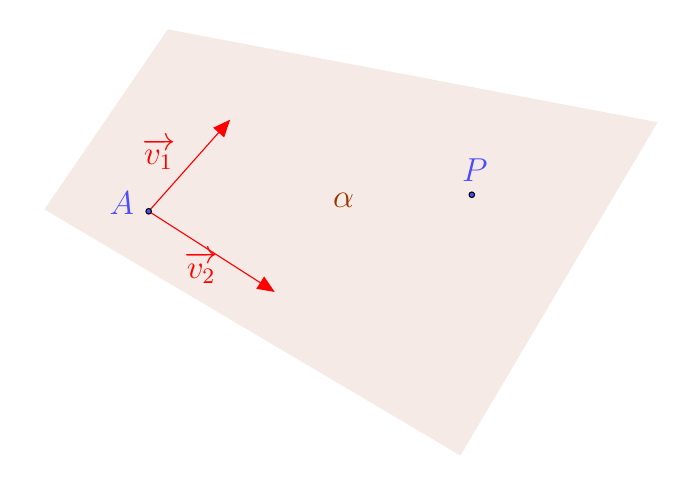
\begin{tikzpicture}[line cap=round,line join=round,>=triangle 45,x=1.0cm,y=1.0cm]
            \clip(-7.074069031825274,-1.3712809724967931) rectangle (0.9979116835037547,4.097030775256176);
            \fill[line width=2.pt,color=zzttqq,fill=zzttqq,fill opacity=0.10000000149011612] (-5.294585710234906,4.075382087127169) -- (-6.861727385744659,1.7892939728526365) -- (-1.578682768304567,-1.3369113282931022) -- (0.9255126925615329,2.8959868055579756) -- cycle;
            \draw [->,line width=0.4pt,color=ffqqqq] (-5.536927206447755,1.7650598232313515) -- (-4.50293682260627,2.9282990050530215);
            \draw [->,line width=0.4pt,color=ffqqqq] (-5.536927206447755,1.7650598232313515) -- (-3.9363141221823366,0.7407861620404246);
            \begin{scriptsize}
                \draw[color=zzttqq] (-3.0623553078910724,1.9090991603117302) node {$\alpha$};
                \draw [fill=ududff] (-5.536927206447755,1.7650598232313515) circle (1.0pt);
                \draw[color=ududff] (-5.635678483304236,1.872684209716261) node[anchor=east] {$A$};
                \draw [fill=ududff] (-1.4332778705768572,1.975089119949153) circle (1.0pt);
                \draw[color=ududff] (-1.3933367389320628,2.048689804261029) node[anchor=south] {$P$};
                \draw[color=ffqqqq] (-5.110696278886221,2.4947729490555277) node[anchor=east] {$\vec{v_{1}}$};
                \draw[color=ffqqqq] (-4.570541178386759,1.3416328468656675) node[anchor=north east] {$\vec{v_{2}}$};
            \end{scriptsize}
        \end{tikzpicture}
    }
\end{minipage}
\begin{minipage}{.49\linewidth}
    \setlength{\parskip}{.3em}

    Tout point $P \in \pi$ peut se décrire:

    \begin{center}
        \cfbox{red}{ $\exists x, y \in \mathbb{R} \tq \vec{AP} = x \cdot \vec{v_{1}} + y \cdot \vec{v_{2}}$}
    \end{center}

    $(x, y)$: coordonnées de $P$ sur $\pi$ relativement au repère $(A,
    \vec{v_{1}}, \vec{v_{2}})$
\end{minipage}

De même on définit un repère dans l'espace $(A, \vec{v_{1}}, \vec{v_{2}},
\vec{v_{3}})$ où $\vec{v_{1}}, \vec{v_{2}}, \vec{v_{3}}$ sont non-complanaires,
non-nuls (le triplet $(\vec{v_{1}}, \vec{v_{2}}, \vec{v_{3}})$ doit former un
parallélépipède non-dégénéré, de volume "positif")

\pagebreak

\paragraph{Changement de repère:}

(dans le plan)

\paragraph{Exemple}

$A, B, C:$ triangle

\begin{minipage}{.5\linewidth}
    \resizebox{\textwidth}{!}{
        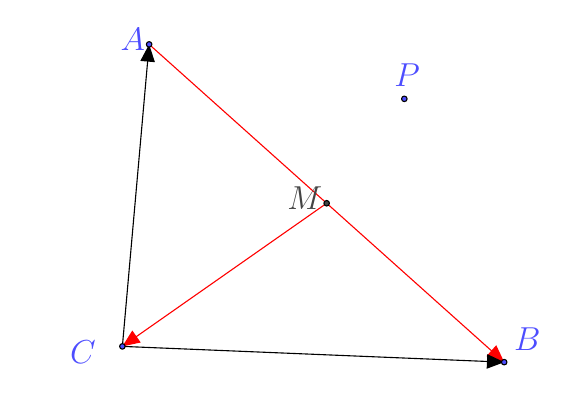
\begin{tikzpicture}[line cap=round,line join=round,>=triangle 45,x=1.0cm,y=1.0cm]
            \clip(-6.15872959185734,-0.7685282709737155) rectangle (0.512328850563343,3.7507376362601406);
            \draw [->,line width=0.4pt,color=ffqqqq] (-4.616059866631097,3.53866819945898) -- (-0.10667515122548199,-0.4973221582055305);
            \draw [->,line width=0.4pt] (-4.955932738855477,-0.2970399299304497) -- (-4.616059866631097,3.53866819945898);
            \draw [->,line width=0.4pt] (-4.955932738855477,-0.2970399299304497) -- (-0.10667515122548199,-0.4973221582055307);
            \draw [->,line width=0.4pt,color=ffqqqq] (-2.3613675089282893,1.5206730206267247) -- (-4.955932738855477,-0.2970399299304498);
            \begin{scriptsize}
                \draw [fill=ududff] (-4.616059866631097,3.53866819945898) circle (1.0pt);
                \draw[color=ududff] (-4.5787420660208635,3.6027705505072003) node[anchor=east] {$A$};
                \draw [fill=ududff] (-0.10667515122548216,-0.4973221582055307) circle (1.0pt);
                \draw[color=ududff] (-0.06950782561771017,-0.4349753488526817) node[anchor=south west] {$B$};
                \draw [fill=ududff] (-4.955932738855477,-0.2970399299304497) circle (1.0pt);
                \draw[color=ududff] (-5.2057212429401005,-0.374785347868435) node[anchor=east] {$C$};
                \draw [fill=uuuuuu] (-2.3613675089282893,1.5206730206267247) circle (1.0pt);
                \draw[color=uuuuuu] (-2.326632862526964,1.5813896841195825) node[anchor=east] {$M$};
                \draw [fill=ududff] (-1.3751292636343293,2.846784138145064) circle (1.0pt);
                \draw[color=ududff] (-1.338513679702246,2.9105855391883635) node[anchor=south] {$P$};
            \end{scriptsize}
        \end{tikzpicture}
    }
\end{minipage}
\begin{minipage}{.49\linewidth}
    \setlength{\parskip}{.3em}

    \textbf{Repère 1:} $(C, \vec{CB}, \vec{CA})$

    Si $P$ est dans le plan,

    $$\exists (x, y) \tq \vec{CP} = x \cdot \vec{CB} + y \cdot \vec{CA}$$

    Si $M$ est milieu de $AB$, alors 
    
    \textbf{Repère 2:}  $(M, \vec{AB}, \vec{MC})$
\end{minipage}

\paragraph{Question}
\label{par:question}

Coordonnées de $P, (x', y')$, relativement au repère 2?

$$\vec{MP} = x' \vec{AB} + y' \vec{MC}$$

$(x', y')$ en fonction de $(x, y)$


\[
    \begin{split}
        \vec{MP} &= \vec{MC} + \vec{CP} = \vec{MC} + x \cdot \vec{CB} + y
        \cdot \vec{CA} \implies \\
        \vec{CA} &= \vec{CM} + \vec{MA} = - \vec{MC} - \frac{1}{2} \vec{AB}\\
        \vec{CB} &= \vec{CM} + \vec{MB} = - \vec{MC} + \frac{1}{2} \vec{AB}\\
        \implies & (1 - x - y) \cdot \vec{MC} + \left(\frac{x}{2} - \frac{y}{2}\right)
        \cdot \vec{AB}\\
        \implies & \left\{\begin{array}{l}x' = \frac{x}{2} - \frac{y}{2} \\ y'=
        1 - x - y\end{array}\right.
    \end{split}
\]


\paragraph{Application}
\label{par:application}

Intersection entre deux droites.


\begin{minipage}{.5\linewidth}
    \resizebox{\textwidth}{!}{
        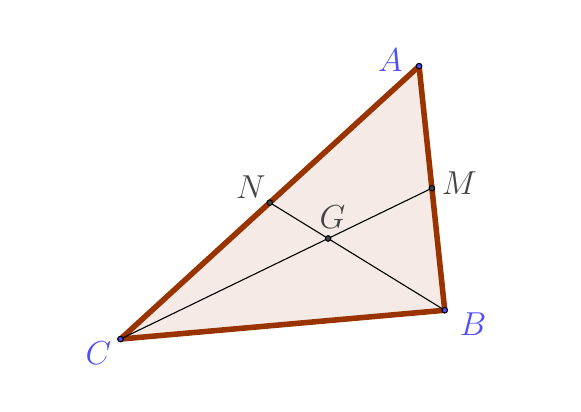
\begin{tikzpicture}[line cap=round,line join=round,>=triangle 45,x=1.0cm,y=1.0cm]
            \clip(-6.7405662680383935,-0.8063750140168409) rectangle (-0.06950782561771017,3.7128908932170166);
            \fill[line width=2.pt,color=zzttqq,fill=zzttqq,fill opacity=0.10000000149011612] (-1.7698753534226812,3.224075127647982) -- (-1.443846181424678,0.12429007695927717) -- (-5.561845415430227,-0.24186576236155685) -- cycle;
            \draw [line width=2.pt,color=zzttqq] (-1.7698753534226812,3.224075127647982)-- (-1.443846181424678,0.12429007695927717);
            \draw [line width=2.pt,color=zzttqq] (-1.443846181424678,0.12429007695927717)-- (-5.561845415430227,-0.24186576236155685);
            \draw [line width=2.pt,color=zzttqq] (-5.561845415430227,-0.24186576236155685)-- (-1.7698753534226812,3.224075127647982);
            \draw [line width=0.4pt] (-5.561845415430227,-0.24186576236155685)-- (-1.6068607674236794,1.6741826023036295);
            \draw [line width=0.4pt] (-3.665860384426454,1.4911046826432126)-- (-1.443846181424678,0.12429007695927717);
            \begin{scriptsize}
            \draw [fill=ududff] (-1.7698753534226812,3.224075127647982) circle (1.0pt);
            \draw[color=ududff] (-2.136031192743517,3.29908463645032) node {$A$};
            \draw [fill=ududff] (-1.443846181424678,0.12429007695927717) circle (1.0pt);
            \draw[color=ududff] (-1.0827061755191985,-0.04647625159072613) node {$B$};
            \draw [fill=ududff] (-5.561845415430227,-0.24186576236155685) circle (1.0pt);
            \draw[color=ududff] (-5.842732086690047,-0.4226637577422681) node {$C$};
            \draw [fill=uuuuuu] (-3.665860384426454,1.4911046826432126) circle (1.0pt);
            \draw[color=uuuuuu] (-3.906620388363443,1.6839862767063667) node {$N$};
            \draw [fill=uuuuuu] (-1.6068607674236794,1.6741826023036295) circle (1.0pt);
            \draw[color=uuuuuu] (-1.5692420168085266,1.7391604442752595) node [anchor=west]{$M$};
            \draw [fill=uuuuuu] (-2.925188983425862,1.0354998140819007) circle (1.0pt);
            \draw[color=uuuuuu] (-2.868342871385186,1.3077987705548249) node {$G$};
            \end{scriptsize}
        \end{tikzpicture}
    }
\end{minipage}
\begin{minipage}{.49\linewidth}
    \setlength{\parskip}{.3em}

    $M$: milieu de $AB$

    $N$: milieu de $AC$

    \textbf{But}: calculer le point d'intersection

    $$G := (NB)\cap(MC)$$
\end{minipage}

\begin{itemize}
    \item Exprimons $G$ dans $(C, \vec{CM})$: $\vec{CG} = \lambda \vec{CM}$
    \item Exprimons $G$ dans $(B, \vec{BN})$: $\vec{BG} = \mu \vec{BN}$
    \item Exprimons les coordonnées de $G$ dans $(C, \vec{CB}, \vec{CA})$, en
        fonction de \cfbox{red}{$\lambda$}:

        \[
            \begin{split}
                \vec{CG} & = \lambda \vec{GM} = \lambda (\vec{CB} + \vec{BM})\\
                & = \lambda \vec{CB} + \frac{\lambda}{2} \vec{BA}\\
                & = \lambda \vec{CB} + \frac{\lambda}{2} ( - \vec{CB} +
                \vec{CA}) \\
                & = {\color{red} \frac{\lambda}{2}} \cdot \vec{CB} + {\color{red} \frac{\lambda}{2}} \vec{CA}
            \end{split}
        \]

    \item Exprimons les coordonnées de $G$ dans $(C, \vec{CB}, \vec{CA})$, en
        fonction de \cfbox{blue}{$\mu$}:
        \[
            \begin{split}
                \vec{CG} & = \vec{CB} + \vec{BG}\\
                \vec{CG} & = \vec{CB} + \mu \vec{BN}\\
                & = \vec{CB} + \mu \cdot (-\vec{CB} + \frac{1}{2} \vec{CA})\\
                & ={\color{blue}1-\mu} \cdot \vec{CB} + {\color{blue}\frac{\mu}{2}} \vec{CA}
            \end{split}
        \]
\end{itemize}
Donc

$$\left\{\begin{array}{l}\frac{\lambda}{2} = 1 - \mu \implies \frac{\lambda}{2}
    = 1 - \lambda \implies \frac{3}{2} \lambda = 1 \implies \lambda =
    \mu = \frac{2}{3}\\ \frac{\lambda}{2} = \frac{\mu}{2} \implies
    \lambda = \mu \end{array}\right.$$

Donc

$$(C, \vec{CB}, \vec{CA}): \vec{CG} = \frac{1}{3}\vec{CB} + \frac{1}{3}\vec{CA}$$


\markDate{11/03/2019}
\section{Droites et plans}
\label{sec:droites_et_plans}

\subsection{Représentation paramétrique}
\label{sub:representation_parametrique}

\paragraph{Droite}


\begin{center}
    \begin{minipage}{.5\linewidth}
        \resizebox{\textwidth}{!}{
            \begin{tikzpicture}[line cap=round,line join=round,>=triangle 45,x=1.0cm,y=1.0cm]
            \clip(0.5,0.1) rectangle (4.7,4.);
            \draw [line width=0.4pt,color=qqqqff,domain=0.5:4.3]  plot(\x,{(--0.3758304883222099--2.1132091315346555*\x)/2.500630805649342}) node [anchor=north]{$d$};
            \draw [->,line width=0.8pt,color=ffqqqq] (1.2484245114535142,1.2053009021356968) -- (2.377123192130964,2.1591307731307254) node [anchor=south east, midway]{$\vec v$};
            \begin{scriptsize}
            \draw [fill=ududff] (1.2484245114535142,1.2053009021356968) circle (0.5pt) node [anchor=south east]{$M$};
            \draw [fill=ududff] (3.749055317102856,3.318510033670352) circle (0.5pt)node [anchor=south]{$P$};;
            \draw [fill=ududff] (2.04087793577901,0.5537280865791782) circle (0.5pt)node [anchor=west]{$A$};
            \end{scriptsize}
            \end{tikzpicture}
        }
    \end{minipage}
    \begin{minipage}{.49\linewidth}
        \setlength{\parskip}{.3em}
        $$\forall P \in d, \exists \lambda \in \mathbb{R} \tq \vec{MP} = \lambda \vec v$$


        $\vec{MP}:$  dans le repère $(A, \vec v)$

        \vspace{.5cm}
        Si $A \notin d$, dans le repère $(A, \vec v)$ 

        $$ \vec{AP} = \vec{AM} + \vec{MP}\\ $$
        \begin{highlightBox}[frametitle={Représentation paramétrique de $d$}]
            $$ \vec{AP} = \vec{AM} + \lambda \cdot \vec v, \quad (\lambda \in \mathbb{R})$$
        \end{highlightBox}
        $${\color{red} \lambda: \text{ paramètre } }$$
    \end{minipage}
\end{center}

\paragraph{Plan}
\begin{center}
    \begin{minipage}{.5\linewidth}
        \resizebox{\textwidth}{!}{
            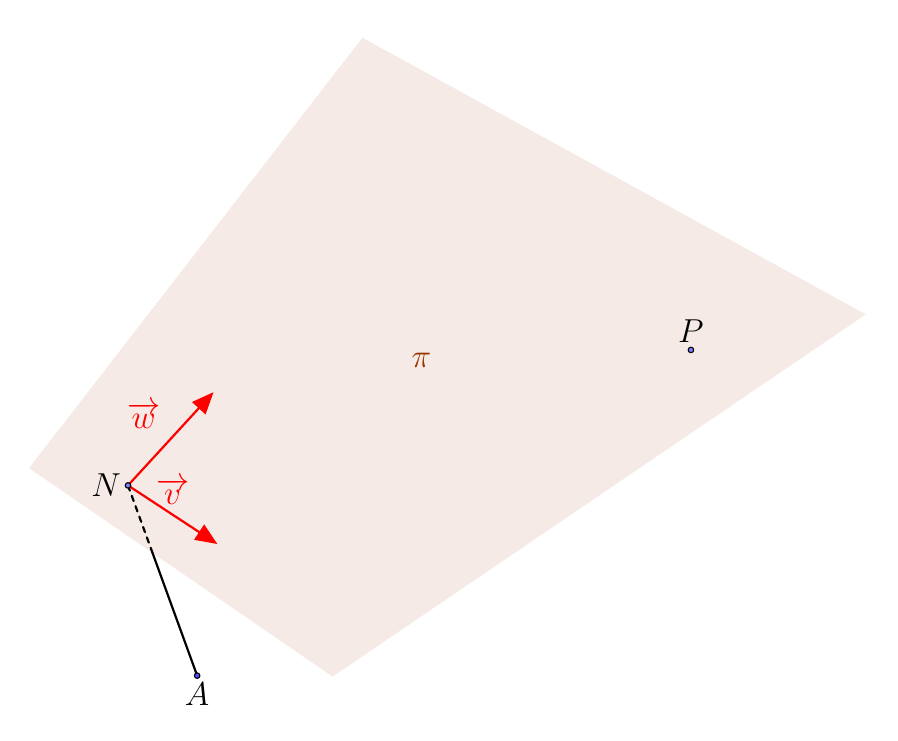
\begin{tikzpicture}[line cap=round,line join=round,>=triangle 45,x=1.0cm,y=1.0cm]
            \clip(0.,1.) rectangle (10.7,9.7);
            \fill[line width=0.pt,color=zzttqq,fill=zzttqq,fill opacity=0.10000000149011612] (0.01729512144772405,4.106287947867099) -- (3.8727544623744996,1.4587098561547247) -- (10.644209950394627,6.058419259728757) -- (4.250979904047695,9.572255621079742) -- cycle;
            \draw [->,line width=0.8pt,color=ffqqqq] (1.2739796534586667,3.886673175282662) -- (2.359852695681714,5.070152783098793)node [midway, anchor=south east]{$\vec w$};
            \draw [->,line width=0.8pt,color=ffqqqq] (1.2739796534586667,3.886673175282662) -- (2.4086559784782557,3.142423112635405) node [midway, anchor=south]{$\vec v$};
            \draw [line width=0.8pt,dash pattern=on 2pt off 2pt] (1.2739796534586667,3.886673175282662)-- (1.5857929591483795,3.0291865846359527);
            \draw [line width=0.8pt] (1.5857929591483795,3.0291865846359527)-- (2.152438743796413,1.47091067685386);
            \begin{scriptsize}
            \draw[color=zzttqq] (5.001684760297062,5.479761812597626) node {$\pi$};
            \draw [fill=xdxdff] (1.2739796534586667,3.886673175282662) circle (1.0pt) node [anchor = east]{$N$};
            \draw [fill=xdxdff] (8.42366058315199,5.606988893860749) circle (1.0pt)node [anchor = south]{$P$};
            \draw [fill=ududff] (2.152438743796413,1.47091067685386) circle (1.0pt)node [anchor = north]{$A$};
            \end{scriptsize}
            \end{tikzpicture}
        }
    \end{minipage}
    \begin{minipage}{.49\linewidth}
        \setlength{\parskip}{.3em}
        $$\forall P \in \pi, \exists \lambda, \mu \in \mathbb{R} \tq \vec{NP}
        = \lambda \cdot \vec v + \mu \cdot \vec w$$
        Si $A \notin \pi$ 

        \begin{highlightBox}[frametitle={Représentation paramétrique de $\pi$}]
            $$ \vec{AP} = \vec{AN} + \lambda \cdot \vec v + \mu \cdot \vec w, \quad (\lambda,\mu \in \mathbb{R})$$
        \end{highlightBox}

    \end{minipage}
\end{center}

\paragraph{Exemple:}

Un cube

\begin{center}
    \begin{minipage}{.49\linewidth}
        \resizebox{\textwidth}{!}{
            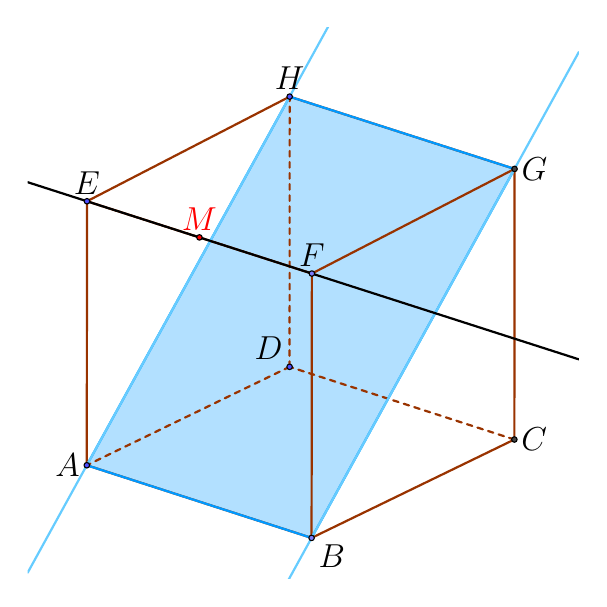
\begin{tikzpicture}[line cap=round,line join=round,>=triangle 45,x=1.0cm,y=1.0cm]
            \clip(0.,0.5) rectangle (7.,7.5);
            \fill[line width=0.8pt,color=qqzzff,fill=qqzzff,fill opacity=0.3] (3.3270471950372813,6.624074525030866) -- (6.183164753311687,5.706146154559268) -- (3.6054247765286216,1.0200422888889933) -- (0.7508793229571764,1.9428479312073481) -- cycle;
            \draw [line width=0.8pt,dash pattern=on 2pt off 2pt,color=zzttqq] (3.32634292132255,3.192511552199415)-- (0.7508793229571764,1.9428479312073481);
            \draw [line width=0.8pt,color=zzttqq] (0.7508793229571764,1.9428479312073481)-- (3.6054247765286216,1.0200422888889933);
            \draw [line width=0.8pt,color=zzttqq] (3.6054247765286216,1.0200422888889933)-- (6.1808883748939945,2.2697059098810604);
            \draw [line width=0.8pt,dash pattern=on 2pt off 2pt,color=zzttqq] (6.1808883748939945,2.2697059098810604)-- (3.32634292132255,3.192511552199415);
            \draw [line width=0.8pt,color=zzttqq] (3.3270471950372813,6.624074525030866)-- (0.7532106512585628,5.295318540600879);
            \draw [line width=0.8pt,color=zzttqq] (0.7532106512585628,5.295318540600879)-- (3.6093282095329693,4.3773901701292806);
            \draw [line width=0.8pt,color=zzttqq] (3.6093282095329693,4.3773901701292806)-- (6.183164753311687,5.706146154559268);
            \draw [line width=0.8pt,color=zzttqq] (6.183164753311687,5.706146154559268)-- (3.3270471950372813,6.624074525030866);
            \draw [line width=0.8pt,color=zzttqq] (0.7508793229571764,1.9428479312073481)-- (0.7532106512585628,5.295318540600879);
            \draw [line width=0.8pt,color=zzttqq] (3.6093282095329693,4.3773901701292806)-- (3.6054247765286216,1.0200422888889933);
            \draw [line width=0.8pt,dash pattern=on 2pt off 2pt,color=zzttqq] (3.32634292132255,3.192511552199415)-- (3.3270471950372813,6.624074525030866);
            \draw [line width=0.8pt,color=zzttqq] (6.1808883748939945,2.2697059098810604)-- (6.183164753311687,5.706146154559268);
            \draw [line width=0.8pt,color=qqzzff] (3.3270471950372813,6.624074525030866)-- (6.183164753311687,5.706146154559268);
            \draw [line width=0.8pt,color=qqzzff] (6.183164753311687,5.706146154559268)-- (3.6054247765286216,1.0200422888889933);
            \draw [line width=0.8pt,color=qqzzff] (3.6054247765286216,1.0200422888889933)-- (0.7508793229571764,1.9428479312073481);
            \draw [line width=0.8pt,color=qqzzff] (0.7508793229571764,1.9428479312073481)-- (3.3270471950372813,6.624074525030866);
            \draw [line width=0.8pt,color=wwccff,domain=0.:7.] plot(\x,{(-1.4900661653343352-4.681226593823518*\x)/-2.576167872080105});
            \draw [line width=0.8pt,color=wwccff,domain=0.:7.] plot(\x,{(-14.2659911965957--4.686103865670274*\x)/2.5777399767830658});
            \draw [line width=0.8pt,domain=0.:7.] plot(\x,{(--15.8154456861978-0.9179283704715981*\x)/2.8561175582744065});
            \begin{scriptsize}
            \draw [fill=ududff] (3.32634292132255,3.192511552199415) circle (1.0pt) node [anchor=south east]{$D$};
            \draw [fill=ududff] (0.7508793229571764,1.9428479312073481) circle (1.0pt)node [anchor=east]{$A$};
            \draw [fill=xdxdff] (3.6054247765286216,1.0200422888889933) circle (1.0pt)node [anchor=north west]{$B$};
            \draw [fill=uuuuuu] (6.1808883748939945,2.2697059098810604) circle (1.0pt)node [anchor=west]{$C$};
            \draw [fill=ududff] (3.3270471950372813,6.624074525030866) circle (1.0pt)node [anchor=south]{$H$};
            \draw [fill=ududff] (0.7532106512585628,5.295318540600879) circle (1.0pt)node [anchor=south]{$E$};
            \draw [fill=xdxdff] (3.6093282095329693,4.3773901701292806) circle (1.0pt)node [anchor=south]{$F$};
            \draw [fill=uuuuuu] (6.183164753311687,5.706146154559268) circle (1.0pt)node [anchor=west]{$G$};
            \draw [fill=ffqqqq] (2.181269430395766,4.83635435536508) circle (1.0pt)node [anchor=south , color = ffqqqq]{$M$};
            \end{scriptsize}
            \end{tikzpicture}
        }
    \end{minipage}
    \begin{minipage}{.50\linewidth}
        \setlength{\parskip}{.3em}
        \textbf{Droite $EF$:}

        \begin{itemize}
        \item \textbf{Repère:} $(E, \vec{EF})$
            \begin{center}
                \cfbox{black}{ $\vec{EP} = \lambda \cdot \vec{EF}, \quad (\lambda
            \in \mathbb{R})$ }
            \end{center}

        \item \textbf{Repère:} $(A, \vec{AB})$
                \begin{equation}
                    \label{eq:1.5}
                    \cfbox{black}{$\vec{AP} = \vec{AE} + \lambda \cdot \vec{AB}, \quad (\lambda
                    \in \mathbb{R})$}
                \end{equation}
        \end{itemize}
    \end{minipage}
\end{center}

Si $M$ est le milieu de $\vec{EF}$, comment décrire le segment $MF$?
$\to$ On restreint les valeurs du paramètre.

Dans l'équation $ \eqref{eq:1.5} $, avec:

\begin{itemize}
    \item $\lambda = 0, \quad P=E$ 
    \item $\lambda = 1, \quad P=F$ 
    \item $\lambda = \frac{1}{2}, \quad P=M$ 
\end{itemize}

Segment $MF$ c'est l'ensemble des $P$ associés aux valeurs $\lambda \in [\ \frac{1}{2}; 1\ ]$ 

\paragraph{Plan $ABGH$:}

\begin{center}
    \cfbox{black}{ $\vec{AP} = \lambda \cdot \vec{AB} + \mu \cdot \vec{AH},
\quad (\lambda, \mu \in \mathbb{R})$ }
\end{center}

Por ne garder que le rectangle $[ABGH]$: restreindre les valeurs de $\lambda$ et
$\mu$: $\lambda \in [0, 1], \mu \in [0, 1]$ 


\paragraph{Équations paramétriques en composantes:}
\label{par:equations_parametriques_en_composantes_}

Dans un repère de l'espace $(A, \vec{e_{1}}, \vec{e_{2}}, \vec{e_{3}})$

\begin{center}
    \begin{minipage}{.39\linewidth}
        \resizebox{\textwidth}{!}{
            \begin{tikzpicture}[line cap=round,line join=round,>=triangle 45,x=1.0cm,y=1.0cm]
            \clip(1.5,0.) rectangle (9.5,6.);
            \draw [->,line width=.7pt,color=qqqqff] (5.236373227908101,0.8629953740577189) -- (1.894120650347376,4.943798146659945)node [midway, anchor=north east]{$\vec{e_3}$};
            \draw [->,line width=.7pt,color=qqqqff] (5.236373227908101,0.8629953740577189) -- (5.6494606251347,2.6905941617875504)node [midway, anchor=east]{$\vec{e_1}$};
            \draw [->,line width=.7pt,color=qqqqff] (5.236373227908101,0.8629953740577189) -- (8.966677602863504,0.7252995749821838)node [midway, anchor=north]{$\vec{e_2}$};
            \draw [->,line width=.7pt,color=ffqqqq] (5.236373227908101,0.8629953740577189) -- (6.988865216142188,5.381921143718472)node [midway, anchor=east]{$\vec v$};
            \draw [fill=ududff] (5.236373227908101,0.8629953740577189) circle (1.0pt);
            \end{tikzpicture}
        }
    \end{minipage}
    \begin{minipage}{.6\linewidth}
        \setlength{\parskip}{.3em}

        Soit $\vec v$ quelconque:
        $$\vec v = \alpha \cdot \vec{e_{1}} + \beta \cdot \vec{e_{2}} + \gamma
        \cdot \vec{e_{3}}$$

        $\alpha, \beta, \gamma:$ \textbf{composantes} de $\vec v$ relativement
        au repère

        $$\vec v= \myVector{\alpha}{\beta}{\gamma} \quad \text{ plutôt: }  \quad \vec v|_{(\vec{e_{1}}, \vec{e_{2}}, \vec{e_{3}})} = \myVector{\alpha}{\beta}{\gamma} $$
    \end{minipage}
\end{center}

Utile si $\vec v = \myVector{\alpha}{\beta}{\gamma}$  et $\vec w = \myVector{\mu}{\nu}{\delta}$,
alors:

\begin{itemize}
    \item $\vec v + \vec w  = \myVector{\alpha + \mu}{\beta + \nu}{\gamma + \delta}$ 
    \item si $t \in \mathbb{R}, \quad t \cdot \vec v = \myVector{t \cdot \alpha}{t \cdot \beta}{t \cdot \gamma}$ 
\end{itemize}

Si $d$ est la droite $(B, \vec w)$:

\begin{center}
    \begin{minipage}{.5\linewidth}
        \resizebox{\textwidth}{!}{
            \begin{tikzpicture}[line cap=round,line join=round,>=triangle 45,x=1.0cm,y=1.0cm]
                \clip(1.5,0) rectangle (9.5,7.5);
                \draw [->,line width=.7pt,color=qqqqff] (5.236373227908101,0.8629953740577189) -- (1.894120650347376,4.943798146659945)node [midway, anchor=north east]{$\vec{e_3}$};
                \draw [->,line width=.7pt,color=qqqqff] (5.236373227908101,0.8629953740577189) -- (5.6494606251347,2.6905941617875504)node [midway, anchor=east]{$\vec{e_1}$};
                \draw [->,line width=.7pt,color=qqqqff] (5.236373227908101,0.8629953740577189) -- (8.966677602863504,0.7252995749821838)node [midway, anchor=north]{$\vec{e_2}$};
                \draw [->,line width=.7pt,color=ffqqqq] (5.236373227908101,0.8629953740577189) -- (6.988865216142188,5.381921143718472)node [midway, anchor=east]{$\vec v$};
                \draw [fill=ududff] (5.236373227908101,0.8629953740577189) circle (1.0pt) node [anchor=north east] {$A$};
                \draw [line width=0.4pt,domain=0.80507205765905:16.627571151429702] plot(\x,{(--58.21196722825283-3.317216977728816*\x)/6.509255956298053});
                \draw [->,line width=.8pt,color=qqzzqq] (4.973499429672997,6.40838073682702) -- (6.15553253698108,5.805998480218092) node [midway, anchor = south]{$\vec w$};
                \draw [fill=ududff] (6.988865216142188,5.381921143718472) circle (1.0pt)node [anchor=south]{$P$};
                \draw [fill=ududff] (4.973499429672997,6.40838073682702) circle (1.0pt) node [anchor=south]{$B$};
                \draw[color=black] (9.2,4.7) node {$d$};
                \draw[color=qqzzqq] (5.949887823117703,6.3896040369530835);
            \end{tikzpicture} 
        }
    \end{minipage}
    \begin{minipage}{.49\linewidth}
        \setlength{\parskip}{.3em}
        $$\vec{AP} = \vec{AB} + \lambda \cdot \vec w, \quad (\lambda \in \mathbb{R})$$

        (relativement au repère $(A, \vec{e_{1}}, \vec{e_{2}}, \vec{e_{3}})$)

        \[
            \begin{split}
                \vec{AP} &= \myVector{x}{y}{z}, \quad P (x, y, z)\\
                \vec{AB} &= \myVector{x_{B}}{y_{B}}{z_{B}}, \quad B(x_{B}, y_{B}, z_{B})\\
                \vec w &= \myVector{w_{1}}{w_{2}}{w_{3}}
            \end{split}
        \]
    \end{minipage}
\end{center}

En composantes:

$$\myVector{x}{y}{z} = \myVector{x_{B}}{y_{B}}{z_{B}} + \lambda \cdot \myVector{w_{1}}{w_{2}}{w_{3}},
\quad (\lambda \in \mathbb{R})$$

$$\left.
\begin{array}{l}
    x = x_{B} + \lambda \cdot w_{1} \\
    y = y_{B} + \lambda \cdot w_{2} \\
    z = z_{B} + \lambda \cdot w_{3} \\
\end{array}
\right\} \longrightarrow \text{ \textbf{équation paramétrique en composantes}  }$$

\paragraph{Exercice:}

Dans un repère du plan: $(A, \vec{e_{1}}, \vec{e_{2}})$

\begin{center}
    \begin{minipage}{.5\linewidth}
        \resizebox{\textwidth}{!}{
            \begin{tikzpicture}[line cap=round,line join=round,>=triangle 45,x=1.0cm,y=1.0cm]
            \clip(0.,-0.5) rectangle (8.5,7.);
            \draw [->,line width=.6pt,color=qqqqff] (2.782884444380373,1.1258691722928327) -- (0.4670914599281897,4.593299749013143)node [midway, anchor=east]{$\vec{e_2}$};
            \draw [->,line width=.6pt,color=qqqqff] (2.782884444380373,1.1258691722928327) -- (5.79967422412621,0.2746587780077002)node [midway, anchor=east]{$\vec{e_1}$};
            \draw [line width=0.8pt,domain=0.:8.5] plot(\x,{(--40.74773514620557-4.343676570837355*\x)/5.26999376461823});
            \begin{scriptsize}
            \draw [fill=ududff] (2.782884444380373,1.1258691722928327) circle (1.0pt) node [anchor=north east]{$A$};
            \draw [fill=ududff] (2.319725847489944,5.820044140777004) circle (1.0pt) node [anchor=south west]{$M$};
            \draw [fill=ududff] (7.5897196121081745,1.4763675699396488) circle (1.0pt) node [anchor=south west]{$P$};
            \draw [fill=xdxdff] (4.597265422409247,3.942832187102423) circle (1.0pt) node [anchor=south west]{$N$};
            \end{scriptsize}
            \end{tikzpicture}
        }
    \end{minipage}
    \begin{minipage}{.49\linewidth}
        \setlength{\parskip}{.3em}
        On a $M (1, 2), \quad N(3, -4)$ 

        $$\vec{AM} = \vec{e_{1}} + 2 \cdot \vec{e_{2}} , \quad \vec{AN} = 3
        \cdot \vec{e_{1}} - 4 \cdot \vec{e_{2}}$$

        Droite $(MN)$ ?

        \[
            \begin{split}
                \vec{AP} &= \vec{AM} + \vec{MP}\\
                &= \vec{AM} + \lambda \cdot \vec{MN} \\
                &\\
                \vec{AM} &= \left(\begin{array}{c}1\\2\end{array}\right)\\
                &\\
                \vec{MN} &= \vec{MA} + \vec{AN} = \vec{AN} - \vec{AM}\\
                &= \left(\begin{array}{c}3\\-4\end{array}\right) - \left(\begin{array}{c}1\\2\end{array}\right)
                    = \left(\begin{array}{c}2\\-6\end{array}\right)\\
            \end{split}
        \]
    \end{minipage}
\end{center}

$$\implies (MN): \myVectorII x y = \myVectorII 1 2 + \lambda \cdot \myVectorII 2 {-6}$$

\paragraph{Est-ce que $H (-1, 3) \in (MN)$ ?}

Si $H \in (MN)$, alors il doit exister $\lambda \in \mathbb{R} \tq$ 

$$\myVectorII {-1} 3 = \myVectorII 1 2 + \lambda \cdot \myVectorII 2 {-6}$$

\begin{equation}
    \label{eq:1.6}
    \left\{
        \begin{array}{l}
        -1 = 1 + 2 \lambda \implies 2 \lambda = -2 \implies \lambda = -1\\
        3 = 2 - 6 \lambda \implies -6 \lambda = 1 \implies \lambda = -\frac{1}{6}
        \end{array}
    \right.\\
\end{equation}

$\implies$ il n'existe aucun $\lambda$ solution de $\eqref{eq:1.6}$

$\implies$ Donc $H \notin (MN)$ 

\textbf{Si $\vec v = \myVectorII 4 1 , \vec w = \myVectorII {-1} 1$ est-ce
que $d = d(M, \vec v), g = g(N, \vec w)$ s'intersectent?  Si oui, quelles sont
les coordonnées du point d'intersection?}

\begin{center}
    \begin{minipage}{.5\linewidth}
        \resizebox{\textwidth}{!}{
            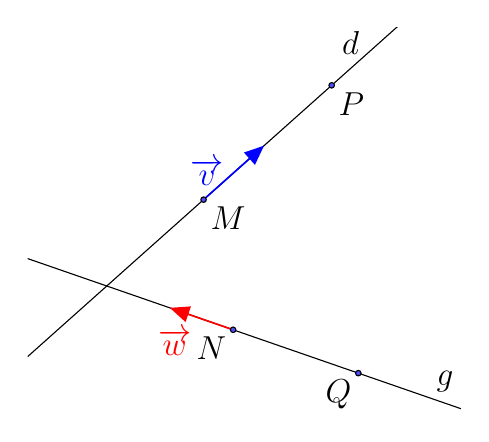
\begin{tikzpicture}[line cap=round,line join=round,>=triangle 45,x=1.0cm,y=1.0cm]
            \clip(1.,0.1) rectangle (6.5,5.);
            \draw [line width=.4pt,domain=1.:6.5] plot(\x,{(--3.8373725369718885-0.550783196302143*\x)/1.5897605893266373});
            \draw [line width=.4pt,domain=1.:6.5] plot(\x,{(-0.11314272380375456--1.4520647902511046*\x)/1.6273139890745143});
            \draw [->,line width=.6pt,color=ffqqqq] (3.609059238833595,1.163422572040704) -- (2.8051587138682548,1.4419392893515313) node [midway, anchor = north east]{$\vec w$};
            \draw [->,line width=.6pt,color=qqqqff] (3.233525241354861,2.815772160947134) -- (4.001401298131226,3.5009538731475813) node [midway, anchor=east]{$\vec v$};
            \begin{scriptsize}
            \draw [fill=ududff] (3.609059238833595,1.163422572040704) circle (1.0pt) node [anchor=north east]{$N$};
            \draw [fill=ududff] (5.198819828160232,0.6126393757385611) circle (1.0pt) node [anchor=north east]{$Q$};
            \draw [fill=ududff] (3.233525241354861,2.815772160947134) circle (1.0pt) node [anchor=north west]{$M$};
            \draw [fill=ududff] (4.8608392304293755,4.267836951198238) circle (1.0pt) node [anchor=north west]{$P$};
            \draw (5.1,4.8) node {$d$};
            \draw (6.3,.5) node {$g$};

            \end{scriptsize}
            \end{tikzpicture}
        }
    \end{minipage}
    \begin{minipage}{.49\linewidth}
        \setlength{\parskip}{.3em}
        
        \[
            \begin{split}
                d &: \vec{AP} = \vec{AM} + \lambda \vec v, \quad (\lambda \in \mathbb{R})\\
                \\
                g &: \vec{AQ} = \vec{AN} + \mu \vec w, \quad (\mu \in \mathbb{R})\\
            \end{split}
        \]
    \end{minipage}
\end{center}

Pour que $d$  et $g$ s'intersectent, il doit exister une paire $(\lambda, \mu)
\tq \vec{AP} = \vec{AQ}$ 

On cherche donc $\lambda, \mu \tq$ 

$$ \myVectorII x y = \underbrace{\myVectorII 1 2 + \lambda \cdot \myVectorII 4 1}_{\vec{AP}}
= \underbrace{\myVectorII 3 {-4} + \mu \myVectorII{-1} 1}_{\vec{AQ}}$$

$$\left\{
    \begin{array}{lll}
        4 \lambda + \mu = 2 &\quad(1)\quad& (1) - (2)\implies 5 \lambda = -4
        \implies \lambda = - \frac{4}{5}\\

        \lambda - \mu = -6  &\quad(2)\quad& (2) \implies \mu = \lambda + 6
        \implies \mu = \frac{-4 + 30}{5} = \frac{26}{5}
    \end{array}
\right.$$

$\longrightarrow$ $d$ et $g$ s'intersectent.

Points d'intersection:

$$\left\{
    \begin{array}{l}
        x = 1 +  4 \lambda = 1 + 4 \cdot - \frac{4}{5} = \frac{5 - 16}{5} = -
        \frac{11}{5}\\
        \\
        y = 2 + \lambda  = 2 + - \frac{4}{5} = \frac{10 -4}{5} = \frac{6}{5}
    \end{array}
\right.$$

\paragraph{Exemple:}

Dans l'espace:

        \[
            \begin{split}
                d &: \myVector x y z = \myVector 1 0 2 + \lambda \cdot
                \myVector 1 1 {-1}, \quad(\lambda \in \mathbb{R})\\
                \\
                g &: \myVector x y z = \myVector 0 {-3} 1 + \mu \cdot
                \myVector 2 1 0, \quad(\mu \in \mathbb{R})\\
            \end{split}
        \]

Est-ce que $d$ et $g$ s'intersectent?
$$ \myVector 1 0 2 + \lambda \cdot \myVector 1 1 {-1} = \myVector 0 {-3} 1 +
\mu \myVector 2 1 0$$
n'a \textbf{pas} de solution $\implies d \cap g = \emptyset$ 

Droites $d$ et $g$ sont \textbf{gauches}: leurs vecteurs directeurs sont
non-colinéaire, et elles ne s'intersectent pas.


\textbf{Intersection de $d$ avec le plan $\pi = \pi (S, \vec{w_{1}} , \vec{w_{2}})$? }

\begin{center}
    \begin{minipage}{.5\linewidth}
        \resizebox{\textwidth}{!}{
            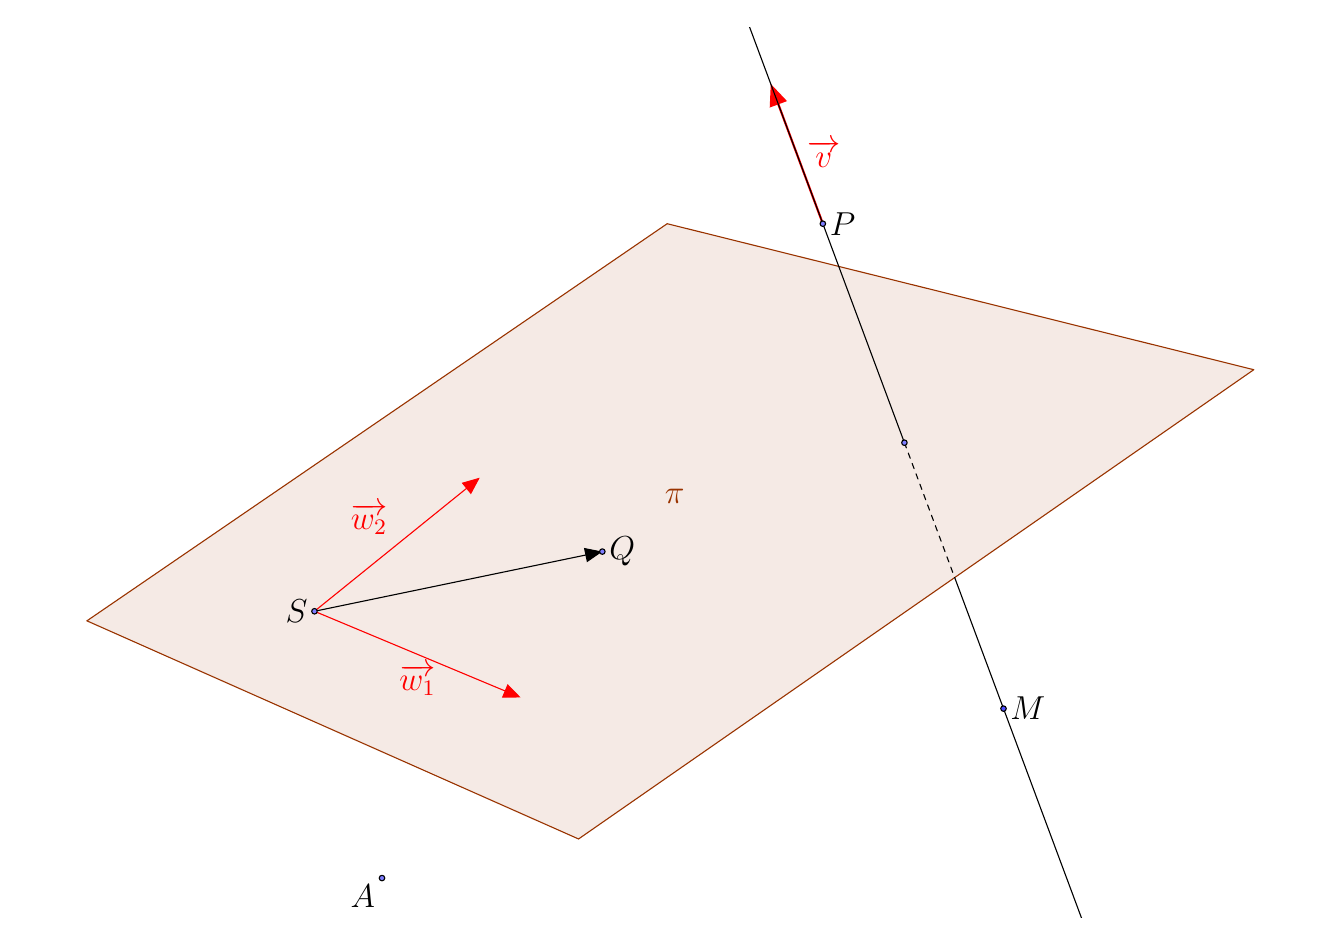
\begin{tikzpicture}[line cap=round,line join=round,>=triangle 45,x=1.0cm,y=1.0cm]
            \clip(0.5,1.5) rectangle (16.8,12.8);
            \fill[line width=0.4pt,color=zzttqq,fill=zzttqq,fill opacity=0.10000000149011612] (8.62179280840684,10.310282555211677) -- (1.2524806882172577,5.266686657849053) -- (7.496080584953404,2.496515357123125) -- (16.07135899302516,8.456168304817783) -- cycle;
            \draw [line width=0.4pt,color=zzttqq] (8.62179280840684,10.310282555211677)-- (1.2524806882172577,5.266686657849053);
            \draw [line width=0.4pt,color=zzttqq] (1.2524806882172577,5.266686657849053)-- (7.496080584953404,2.496515357123125);
            \draw [line width=0.4pt,color=zzttqq] (7.496080584953404,2.496515357123125)-- (16.07135899302516,8.456168304817783);
            \draw [line width=0.4pt,color=zzttqq] (16.07135899302516,8.456168304817783)-- (8.62179280840684,10.310282555211677);
            \draw [->,line width=0.4pt,color=ffqqqq] (4.142228809374071,5.388150466779978) -- (6.241215184672055,7.084463060245083) node [midway, anchor = south
            east]{$\vec{w_2}$};
            \draw [->,line width=0.4pt,color=ffqqqq] (4.142228809374071,5.388150466779978) -- (6.761111447326777,4.293441018624998) node [midway, anchor = north]{$\vec{w_1}$};
            \draw [->,line width=0.8pt,color=ffqqqq] (10.59864735946045,10.310170990023984) -- (9.937319856926434,12.085313233667922) node [midway, anchor = west]{$\vec{v}$};
            \draw [->,line width=0.4pt] (4.142228809374071,5.388150466779978) -- (7.79811403792412,6.146295722988962);
            \draw [line width=0.4pt,domain=0.5:11.634728465296917] plot(\x,{(-40.15764557673799--2.781059810403147*\x)/-1.036081105836466});
            \draw [line width=0.4pt,domain=12.272844304597923:16.8] plot(\x,{(--24.031970075406825-1.6642994174997146*\x)/0.6200331163234214});
            \draw [line width=0.4pt,dash pattern=on 2pt off 2pt] (11.634728465296917,7.529111179620837)-- (12.272844304597923,5.816273926760244);
            \begin{scriptsize}
            \draw[color=zzttqq] (8.718612562799102,6.850050832457418) node {$\pi$};
            \draw [fill=xdxdff] (5,2) circle (1.0pt) node [anchor= north east]{$A$};
            \draw [fill=xdxdff] (4.142228809374071,5.388150466779978) circle (1.0pt) node [anchor= east]{$S$};
            \draw [fill=xdxdff] (7.79811403792412,6.146295722988962) circle (1.0pt) node [anchor= west]{$Q$};
            \draw [fill=xdxdff] (11.634728465296917,7.529111179620837) circle (1.0pt);
            \draw [fill=ududff] (12.892877420921344,4.15197450926053) circle (1.0pt) node [anchor= west]{$M$};
            \draw [fill=xdxdff] (10.59864735946045,10.310170990023984) circle (1.0pt) node [anchor= west]{$P$};
            \end{scriptsize}
            \end{tikzpicture}
        }
    \end{minipage}
    \begin{minipage}{.49\linewidth}
        \setlength{\parskip}{.3em}
        \[
            \begin{split}
                S &\ (0, 0, 2)\\
                M &\ (1, 0, 2)\\
                \vec v & \myVector 1 1 {-1}\\
                \vec{w_{1}} & \myVector 1 1 2, \vec{w_{2}} \myVector 1 {-1} {-1}\\
            \end{split}
        \]
    \end{minipage}
\end{center}

$$\left\{
    \begin{array}{ll}
        d: \vec{AP} = \vec{AM} + \lambda \cdot \vec v  &\lambda \in \mathbb{R}\\
        \pi: \vec{AQ} = \vec{AS} + \alpha \cdot \vec{w_{1}} + \beta \cdot \vec{w_{2}} \quad \quad \quad \quad &\alpha, \beta \in \mathbb{R}\\
    \end{array}
\right.$$

$\longrightarrow$  On cherche $\lambda, \alpha, \beta$  tels que $\vec{AP} =
\vec{AQ}$ 

$$ \myVector102 + \lambda \cdot \myVector 11{-1} = \myVector 002 + \alpha \cdot
\myVector 112 + \beta \cdot \myVector 1{-1}{-1}$$

$$\longrightarrow \alpha = \frac{1}{3}, \quad \beta = \frac{1}{2}, \quad \lambda = - \frac{1}{6}$$


Intersection $I$ :
\[
    \begin{split}
        x &= 1 + \lambda = a - \frac{1}{6} = \frac{5}{6}\\
        y &= \lambda = -\frac{1}{6}\\
        z &= 2 - \lambda = 2 + \frac{1}{6} = \frac{13}{6}\\
    \end{split}
\]

Donc $I (\frac{5}{6}, - \frac{1}{6}, \frac{13}{6})$ 


II Plans dans l'espace

Dans le repère de l'espace 

$$\cfbox{black}{ax + by + cz + d = 0} \rightarrow {\color{red} \text{ n'est \textbf{pas} l'équation
d'un droite dans l'espace}}$$
décrit un plan! En effet: (supposons $c \neq 0$)

$$z = - \frac{d}{c} - \frac{a}{c} x - \frac{b}{c} y$$

Donc tout triplet $(x, y, z)$ qui satisfait (*) peut s'écrire ainsi

\[
    \begin{split}
        \myVector x y z = \myVector 0 0 {-\frac{d}{c}} + x \myVector 1 0
        {-\frac{a}{c}} + y \myVector 0 1 {-\frac{b}{c}}, \quad x, y \in \mathbb{R}
    \end{split}
\]

Plus généralement, comment trouver des directions indépendantes seulement à
partir de l'équation cartésienne du plans $\pi: a x +by +cd = 0$ ?

 $\rightarrow$ On choisit des points (au moins 3)

 \[
     \begin{split}
         A \in \pi& \implies a x_{A} + b y_{A} + c z_{A} + d = 0\\
         B \in \pi& \implies a x_{B} + b y_{B} + c z_{B} + d = 0\\
     \end{split}
 \]

 $$a \underbrace{(x_{B} -x _{A})}_{v_{1}} + b \underbrace{(y_{B} - y_{A})}_{v_{2}} + c \underbrace{(z_{B} - z_{A})}_{v_{3}} = 0$$


 \paragraph{Donc}
 \label{par:donc}
 
 \cfbox{black}{$\vec v = \myVector {v_{1}} {v_{2}} {v_{3}}$  est directeur de $\pi \iff a
 v_{1} + b v_{2} + c v_{3} =0$}

 Plan: \textbf{équation cartésienne $\implies$ équation paramétrique} 

 \begin{itemize}
     \item chercher/choisir un $A (x_{0}, y_{0}, z_{0}) \tq a x_{0} + by_{0} +
         c z_{0} + d = 0$ 
        \item trouver deux directions indépendantes avec $v_{1} + b v_{2} + c v_{3} =0$
 \end{itemize}

\paragraph{Exemple}

Dans un repère : $\myVector x y z = \myVector 1 3 1 +\lambda \myVector 1 1 0 +
\mu \myVector 3 0 1$ 

 look at the paper

Dans la premiere: $x = 1 + (y -3 ) + 3 (z-1)$ 

$$x - y - 3z + 5 =0$$

Dans le cas générale:
$$\myVector x y z = \myVector{x_{0}}{y_{0}}{z_{0}}  +\lambda \myVector{v_{1}}{v_{2}}{v_{3}}+\mu \myVector{u_{1}}{u_{2}}{u_{3}}(**)$$

 $\rightarrow$ Comment obtenir les $a, b, c$ de l'équation cartésienne $a x +
 by+ cz + d =0$ ?

 \textbf{Affirmation:} l'équation cartésienne associé à (**) est de la forme 

 \cfbox{black}{$ \underbrace{(v_{2}u_{3} - v_{3}u_{2})}_{a} x + \underbrace{(-u_{3}u_{1} -
 u_{1}v_{3})}_{b} y +\underbrace{(-v_{2}u_{1} - v_{1}v_{2})}_{c} z = \text{
 cste }  \leftarrow \text{ se trouve en choisissant un point } $}

\paragraph{En effet :} Il suffit de vérifier que 

$$av_{1} + bv_{2} + c v_{3} = 0 \text{ et } au_{1} + bu_{2} + c u_{3} = 0 $$


 missing some shit look at the photos of alessio

\paragraph{En général:}
\label{par:en_general_}

Une droite $d$ (dans l'espace) est décrite par deux \textbf{équations
cartésienne}:

$$d: \left\{\begin{array}{l}a x + b y + c z + d = 0 \leftarrow \text{c'est un
    plan}\alpha! \\ a' x + b' y +c'z + d' = 0 \text{c'est un plan}\beta!\end{array}\right.$$

    $$\implies d =\alpha \cap\beta$$

\Warning Il y a une infinité des paires de plans qui décrivent la même droite!

\paragraph{Équation cartésienne $\implies$ équation paramétrique?}
\label{par:equation_cartesienne_implies_equation_parametrique_}

Si $d$ est donné comme en (\^*), comment trouver un vecteur directeur $\vec v$ ?

 $\vec v$  doit être directeur à la fois pour $\alpha$ \textbf{et} pour $\beta$ !


 \paragraph{Affirmation}
 \label{par:affirmation}
 
 on peut par exemples prendre

 $$\vec v = \myVector {bc'-b'c}{a'c - ac'}{ab'-a'b} = \myVector {v_{1}}{v_{2}}{v_{3}}$$

 \paragraph{Vérifions}
 \label{par:verifions}
 
 $\vec v$ dirige $\alpha$, car 
 $$a v_{1} + b v_{2} + c v_{3} = a(bc' -b'c) - b(a'c - ac') + c (ab' -a'b) = 0 $$

 $\vec v$ dirige $\beta$, car
 $$a' v_{1} + b'v_{2} + c'v_{3} = ( \text{ faire !} ) = 0$$


 \paragraph{Exemple}
 
 $$d : \left\{\begin{array}{l}x + y + z = 1\\2x-y=0 \quad c'=0\end{array}\right.$$

     Pour formule : $\vec v = \myVector {1 \cdot 0 - (-1)1} \ldots \ldots =
     \myVector 1 2 {-3} $  dirige $d$ 

     Donc $A ( 0, 0, 1) \in d$ 

     $$\rightarrow \myVector x y z = \myVector 0 0 1 + t \cdot \myVector 1 2
     {-3}, \quad t \in \mathbb{R}$$
\end{document}
